\documentclass[border=3pt]{standalone}
\usepackage{fontspec}
\newfontfamily\chessfont{Apple Symbols}
\usepackage{tikz}
\usepackage{pgfplots}
\pgfplotsset{compat=1.17}
\definecolor{light}{HTML}{EDEDED}
\definecolor{dark}{HTML}{7389B8}
\definecolor{edge}{HTML}{4A4A4A}
\definecolor{blue2}{HTML}{B9C6E0}
\begin{document}
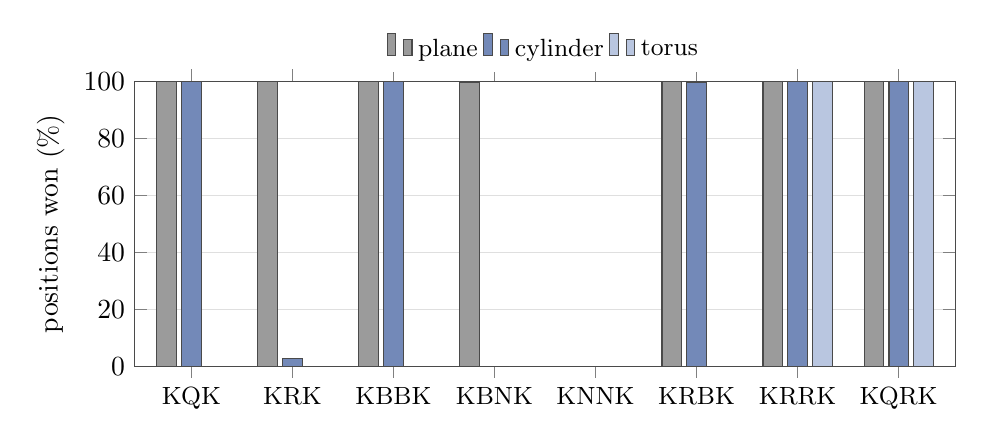
\begin{tikzpicture}\begin{axis}[ybar, bar width=7pt, width=12cm, height=5.2cm,
  ymin=0, ymax=100, ylabel={positions won (\%)}, symbolic x coords={KQK,KRK,KBBK,KBNK,KNNK,KRBK,KRRK,KQRK}, xtick=data,
  x tick label style={font=\small}, ymajorgrids, grid style={gray!25}, enlarge x limits=0.08,
  legend style={at={(0.5,1.03)}, anchor=south, legend columns=3, draw=none, font=\small},
  axis line style={edge}]
\addplot[fill=edge!55, draw=edge] coordinates {(KQK,100) (KRK,100) (KBBK,99.98) (KBNK,99.51) (KNNK,0.0107) (KRBK,100) (KRRK,100) (KQRK,100)};
\addlegendentry{plane}
\addplot[fill=dark, draw=edge] coordinates {(KQK,100) (KRK,2.8) (KBBK,100) (KBNK,0.0245) (KNNK,0.0077) (KRBK,99.74) (KRRK,100) (KQRK,100)};
\addlegendentry{cylinder}
\addplot[fill=blue2, draw=edge] coordinates {(KQK,0) (KRK,0) (KBBK,0) (KBNK,0) (KNNK,0) (KRBK,0.0218) (KRRK,100) (KQRK,100)};
\addlegendentry{torus}
\end{axis}\end{tikzpicture}
\end{document}
